\documentclass[10pt, aspectratio=169]{beamer}

% Tema e Cores
\usetheme{Madrid}
\usecolortheme{default}

% Pacotes de Idioma, Codificação e Gráficos
\usepackage[utf8]{inputenc}
\usepackage[T1]{fontenc}
\usepackage[brazilian]{babel}
\usepackage{amsmath, amssymb}
\usepackage{booktabs}
\usepackage{multirow}
\usepackage{graphicx}
\usepackage{adjustbox}
\usepackage{caption}
\usepackage{orcidlink}
% Pacotes para o Pipeline em TikZ
\usepackage{tikz}
\usetikzlibrary{shapes.geometric, arrows.meta, positioning, calc}

% --- COMANDO PARA INSERIR A LOGO ANTES DO TÍTULO ---
\addtobeamertemplate{title page}{
    \centering
    
\includegraphics[height=2.7cm]{CBIE_2026.jpg}\par
}{}


% Configurações de Título
\title[Proficiência ENADE 2017 via TRI]{Mensuração da Proficiência dos Estudantes de Sistemas de Informação na Prova do ENADE (2017) via Teoria de Resposta ao Item (TRI)}

\author[Valente, Monteiro, Tavares]{\textbf{Mário Diego R. Valente}\inst{1} \orcidlink{0000-0001-7262-3336} \and \textbf{Dionne Cavalcante Monteiro}\inst{1} \orcidlink{0000-0003-0838-3379} \and \textbf{Heliton Ribeiro Tavares}\inst{2} \orcidlink{0000-0003-1725-3364}}

\institute[UFPA]{
  \inst{1} Faculdade de Computação -- Universidade Federal do Pará (UFPA) \and
  \inst{2} Faculdade de Estatística -- Universidade Federal do Pará (UFPA)
}

\date{07/10/2026}

\begin{document}

% --- SLIDE 1: Capa ---
\begin{frame}
    \titlepage
\end{frame}

% --- SLIDE 2: Sumário ---
\begin{frame}{Roteiro da Apresentação}
    \tableofcontents
\end{frame}

% ==========================================
% SEÇÃO 1: INTRODUÇÃO E FUNDAMENTAÇÃO
% ==========================================
\section{Introdução e Fundamentação}

\begin{frame}{Introdução}
    \begin{itemize}
        \item \textbf{Contexto:} O ENADE avalia o rendimento dos concluintes (Lei nº 10.861/2004 - SINAES).
        \item \textbf{Por que 2017?} Último ciclo avaliativo pleno antes das reformulações promovidas pelas novas Diretrizes Curriculares Nacionais (DCNs) da Computação. Funciona como \textit{baseline} histórica.
        \item \textbf{Estrutura do Exame:} Formação Geral (25\% - 10 questões) e Componente Específico (75\% - 30 questões).
        \item \textbf{Problema:} O INEP divulga resultados via Teoria Clássica dos Testes (TCT), que avalia apenas o escore bruto, ignorando o peso, a dificuldade de cada questão e os acertos casuais (chutes).
    \end{itemize}
\end{frame}

\begin{frame}{Objetivos do Estudo}
    \begin{block}{Objetivo Principal}
        Mensurar a proficiência latente dos estudantes concluintes de Sistemas de Informação no ENADE 2017 utilizando a Teoria da Resposta ao Item (TRI).
    \end{block}
    \vspace{0.3cm}
    \textbf{Objetivos Específicos:}
    \begin{itemize}
        \item Calibrar os parâmetros psicométricos dos itens (dificuldade, discriminação e pseudo-acerto).
        \item Classificar os alunos em faixas de desempenho (Básico, Intermediário e Avançado).
        \item Mapear os conteúdos da Computação que representam os maiores gargalos de aprendizagem no país.
    \end{itemize}
\end{frame}

\begin{frame}{Fundamentação Teórica: O Modelo TRI (ML3P)}
    A Teoria de Resposta ao Item (TRI) garante \textbf{invariância}: a dificuldade do item não depende da amostra e a nota do aluno não depende do teste.
    
    \vspace{0.3cm}
    \textbf{Modelo Logístico de 3 Parâmetros (ML3P):}
    $$ P(U_{ij}=1|\theta_{j}) = c_{i} + (1-c_{i})\frac{1}{1+e^{-Da_{i}(\theta_{j}-b_{i})}} $$
    
    Onde:
    \begin{itemize}
        \item $\theta_{j}$: Habilidade latente do estudante.
        \item $a_{i}$: Parâmetro de \textbf{Discriminação} (inclinação da curva).
        \item $b_{i}$: Parâmetro de \textbf{Dificuldade} (escala de proficiência).
        \item $c_{i}$: Parâmetro de \textbf{Acerto Casual} (chute). Esperado $\approx 0,20$.
    \end{itemize}
\end{frame}

% ==========================================
% SEÇÃO 2: TRABALHOS CORRELATOS
% ==========================================
\section{Trabalhos Correlatos}

\begin{frame}{Quadro Síntese da Literatura (Trabalhos Correlatos)}
    \begin{table}[H]
        \centering
        \resizebox{\textwidth}{!}{
        \begin{tabular}{l|l|l|c}
          \hline \hline
        \textbf{Autores (Ano)} & \textbf{Curso Analisado} & \textbf{Edição (ENADE)} & \textbf{Metodologia Principal} \\
          \hline \hline
        Oliveira (2006) & Medicina & 2004 & TRI (Modelo Clássico) \\
        Nogueira (2008) & Formação Geral & 2004, 2005 & TRI (Modelo de Rasch) \\
        Primi et al. (2011) & Psicologia & 2006 & TRI (Modelos Mistos) \\
        Coelho et al. (2014) & Estatística & Não especificado & TRI (Avaliação Paramétrica) \\
        Camargo et al. (2016) & Ciências Contábeis & 2012 & TRI (Modelo de 3 Parâmetros) \\
        Figueiró e Mozzaquatro (2017) & Ciência da Computação & 2014 & TCT e Estatística Descritiva \\
        Lima et al. (2018) & Computação (Geral) & Várias & Classificação Semântica \\
        Araújo (2019) & Cursos Gerais (TI) & 2017 & Data Mining / Machine Learning \\
        Charão et al. (2020) & Ciência da Computação & 2005 a 2017 & TCT e Análise Longitudinal \\
        Cunha et al. (2021) & Ciência da Computação & 2005 a 2014 & Automatização (Scripts Python) \\
        Rendeiro et al. (2022) & Engenharia da Computação & 2014, 2017, 2019 & TCT e Análise Descritiva \\
          \hline \hline
        \textbf{O presente estudo} & \textbf{Sistemas de Informação} & \textbf{2017} & \textbf{TRI (Modelo de 3 Parâmetros)} \\
        \bottomrule
        \end{tabular}}
    \end{table}
\end{frame}

% ==========================================
% SEÇÃO 3: METODOLOGIA
% ==========================================
\section{Metodologia}

\begin{frame}{População, Amostra e Coleta de Dados}
    \begin{itemize}
        \item \textbf{Amostra:} $11.523$ concluintes de Bacharelado em Sistemas de Informação.
        \item \textbf{Base de Dados:} Microdados oficiais do INEP (ENADE 2017).
        \item \textbf{Extração (Data Wrangling):} O vetor de respostas dos alunos foi comparado ao gabarito para gerar uma matriz dicotômica (1 = Acerto, 0 = Erro).
        \item \textbf{Itens Válidos:} $34$ questões objetivas (a Q14 foi anulada pelo INEP e removida).
        \item \textbf{Classificação Pedagógica:} Categorização dos conteúdos da prova em 17 áreas da Computação e divisão na \textbf{Taxonomia de Bloom} (Básico, Intermediário, Avançado).
        \item \textbf{Software:} Processamento realizado no R-Project (v.4.5.5) usando pacotes \texttt{mirt}, \texttt{ltm}, \texttt{irtoys} e \textit{psych}.
    \end{itemize}
\end{frame}


\begin{frame}{Modelagem Não-Supervisionada (TRI)}
    \centering
    \vspace{0.4cm}
    \resizebox{0.95\textwidth}{!}{ % Ajusta o tamanho para caber perfeitamente no slide 16:9
    \begin{tikzpicture}[
        node distance=0.8cm and 0.8cm,
        % Estilos das caixas otimizados para layout horizontal
        inputbox/.style={rectangle, draw=black!70, rounded corners, fill=blue!5, text width=2.8cm, align=center, minimum height=1.8cm, font=\footnotesize},
        modelbox/.style={rectangle, draw=blue!80, thick, rounded corners, fill=blue!15, text width=3.4cm, align=center, minimum height=1.8cm, font=\footnotesize},
        outputbox/.style={rectangle, draw=black!70, rounded corners, fill=green!10, text width=3.2cm, align=center, minimum height=1.4cm, font=\footnotesize},
        arrow/.style={-{Stealth[scale=1.2]}, thick, draw=black!70}
    ]

    % 1. Dados
    \node (data) [inputbox] {\textbf{1. Microdados ENADE} \\ Respostas Brutas \\ (Sistemas de Informação)};

    % 2. Pre-processamento
    \node (prep) [inputbox, right=of data] {\textbf{2. Data Wrangling} \\ Matriz Dicotômica (0/1) \\ Remoção da Q14};

    % 3. Modelo
    \node (model) [modelbox, right=1cm of prep] {\textbf{3. Estimação TRI} \\ (Pacote \texttt{mirt}) \\ Modelo ML3P \\ Algoritmo EM};

    % 4. Saídas (Bifurcação: uma acima e outra abaixo)
    \node (param) [outputbox, above right=0.1cm and 1cm of model] {\textbf{4a. Parâmetros (Itens)} \\ Dificuldade ($b_i$) \\ Discriminação ($a_i$) \\ Acerto Casual ($c_i$)};
    
    \node (theta) [outputbox, below right=0.1cm and 1cm of model] {\textbf{4b. Traço Latente} \\ Proficiência Estimada ($\theta$) \\ \textit{(Variável alvo futura)}};

    % Setas retas (Entrada -> Pre-processamento -> Modelo)
    \draw [arrow] (data) -- (prep);
    \draw [arrow] (prep) -- (model);

    % Setas com quebra de 90 graus (Modelo -> Saídas)
    \draw [arrow] (model.east) -- ++(0.4,0) |- (param.west) node[pos=0.75, above, font=\scriptsize] {Calibração};
    \draw [arrow] (model.east) -- ++(0.4,0) |- (theta.west) node[pos=0.75, below, font=\scriptsize] {Scoring};

    % Caixa pontilhada de destaque
    \draw [dashed, draw=red, thick, rounded corners] 
        ($(model.north west)+(-0.2, 0.6)$) rectangle ($(model.south east)+(0.2, -0.2)$);
    \node[text=red, font=\scriptsize\bfseries, above] at ($(model.north)+(0, 0.25)$) {Extração Não-Supervisionada};

    \end{tikzpicture}
    }
\end{frame}













% ==========================================
% SEÇÃO 4: RESULTADOS DESCRITIVOS (TCT)
% ==========================================
\section{Resultados - TCT}

\begin{frame}{Resultados Descritivos: Escore Bruto}
    Panorama nacional sob a ótica clássica: Severidade na prova e ausência de notas máximas.
    \vspace{0.3cm}
    \begin{table}[H]
        \centering
        \caption{Medidas Estatísticas do Escore Bruto Geral ($n=11.523$)}
        \resizebox{0.8\textwidth}{!}{
        \begin{tabular}{l|c|c|c}
          \hline \hline
        \textbf{Escores (0 a 35)} & \textbf{Formação Geral} & \textbf{Componente Específico} & \textbf{Escore Total} \\
         \hline \hline
        Nº de Itens       & 8       &  27      &  35             \\
        Média             &  3,99   &  10,90   &  14,90          \\
        Mínimo            &  0      &  0       &  0              \\
        Máximo            &  8      &  23      &  30             \\
        1º Quartil (25\%) &  3      &  8       &  12             \\
        3º Quartil (75\%) &  5      &  13      &  18             \\
          \hline \hline
        \end{tabular}}
    \end{table}
\end{frame}

\begin{frame}{Resultados Descritivos: Notas Brutas (0 a 100)}
    \begin{table}[H]
        \centering
        \caption{Medidas Estatísticas da Nota Bruta Geral ($n=11.523$)}
        \resizebox{0.8\textwidth}{!}{
        \begin{tabular}{l|c|c|c}
          \hline \hline
        \textbf{Notas (0 a 100)} & \textbf{Formação Geral} & \textbf{Componente Específico} & \textbf{Nota Final} \\
          \hline \hline
        Mínimo            &  0,00   &  0,00   &  0,00         \\
        Máximo            &  100,00 &  95,50  &  87,30        \\
        Média             & 49,95   &  46,71  &  44,65        \\
        1º Quartil (25\%) &  37,50  &  36,40  &  35,50        \\
        Mediana           &  50,00  & 45,50   &  44,50        \\
        3º Quartil (75\%) &  62,50  &  59,10  &  53,70        \\
          \hline \hline
        \end{tabular}}
    \end{table}
\end{frame}

\begin{frame}{Distribuição de Frequência - Formação Geral}
   % A maioria dos estudantes concentrou-se entre 3 e 5 acertos na Formação Geral (FG).
   % \vspace{0.3cm}
    \begin{table}[H]
        \centering
       % \caption{Frequência dos Escores na Formação Geral (8 Itens)}
        \resizebox{0.6\textwidth}{!}{
        \begin{tabular}{c|c}
        \hline \hline
        \textbf{Nº de Acertos (FG)}  & \textbf{Nº de Alunos (\%)}      \\
        \hline \hline
               0            &  144 (1,25\%)      \\
               1            &  575 (4,99\%)      \\
               2            &  1.475 (12,80\%)  \\
               3            &  2.245 (19,48\%)   \\
               4            &  2.685 (23,29\%)   \\
               5            &  2.256 (19,58\%)   \\
               6            &  1.387 (12,04\%)   \\
               7            &    604 (5,24\%)   \\
               8            &    152 (1,32\%)   \\
       \hline \hline
             \textbf{Total}         &    \textbf{11.523 (100\%)} \\
        \bottomrule
        \end{tabular}}
    \end{table}
\end{frame}

\begin{frame}{Distribuição de Frequência - Componente Específico}
  %  Nenhum aluno gabaritou a prova específica. Apenas 2 alunos alcançaram 23 acertos.
%\vspace{0.3cm}
    \begin{table}[H]
        \centering
       % \caption{Frequência dos Escores no Componente Específico (27 Itens)}
        \resizebox{\textwidth}{!}{
        \begin{tabular}{c|c|c|c}
          \hline \hline
        \textbf{Nº de Acertos (CE)} & \textbf{Nº de Alunos (\%)} & \textbf{Nº de Acertos (CE)} & \textbf{Nº de Alunos (\%)} \\
          \hline \hline
                 0          &     14 (0,12\%)     &     12             &  1.281 (11,26\%)  \\
                 1          &     06 (0,05\%)     &     13             &  1.052 (9,24\%)   \\
                 2          &     31 (0,27\%)     &     14             &  898   (7,89\%)   \\
                 3          &     103 (0,90\%)    &     15             &  643   (5,65\%)   \\
                 4          &     179 (1,57\%)    &     16             &  471   (4,14\%)   \\
                 5          &     357 (3,14\%)    &     17             &  308   (2,71\%)   \\
                 6          &     518 (4,55\%)    &     18             &  198   (1,74\%)   \\
                 7          &     721 (6,33\%)    &     19             &  90    (0,79\%)   \\
                 8          &     979 (8,60\%)    &     20             &  40    (0.35\%)   \\
                 9          &    1.146 (10,07\%)  &     21             &  18    (0,16\%)   \\
                 10         &    1.241 (10,90\%)  &     22             &  02    (0,02\%)   \\
                 11         &    1.225 (10,76\%)  &     23             &  02    (0,02\%)   \\
          \hline \hline
        \end{tabular}}
    \end{table}
\end{frame}

\begin{frame}{Proporção de Acertos e Erros: Parte 1 (Q01 a Q15)}
  %  Avaliação empírica da TCT antes da modelagem. Nota-se altíssimo erro na Q09 e Q10.
    \begin{table}[H]
        \centering
        \resizebox{0.7\textwidth}{!}{
        \begin{tabular}{c|c|c|c|c|c|c}
        \hline \hline
        \textbf{Caderno} & \textbf{Item} & \textbf{Erros (\%)} & \textbf{(n)} & \textbf{Acertos (\%)} & \textbf{(n)} & \textbf{Gabarito} \\
        \hline \hline
               & 01          &  76,60             &  8.827   & 23,40             &  2.696   &  C       \\
               & 02          &  49,97             &  5.758   &  50,03            & 5.765    &  C       \\
               & 03          &  64,55             &  7.438   &  35,45            & 4.085    &  B       \\
               & 04          &  36,74             &  4.233   &  63,26            & 7.290    &  B       \\
               & 05          &  38,37             &  4.421   &  61,63            & 7.102    &  C       \\
               & \textbf{06} &  15,46             &  1.782   & \textbf{84,54}    & 9.741    &  E       \\
               & 07          &  65,17             &  7.510   & 34,83             & 4.013    &  A       \\
        FG     & 08          &  53,54             &  6.169   & 46,46             & 5.354    &  D       \\
        \hline \hline 
               & \textbf{09} & \textbf{82,90}      &  9.552   & 17,10            & 1.971    &  C      \\
               & \textbf{10} &  \textbf{89,60}     &  10.325  & 10,40            &  1.198   &  E      \\
               & 11          &  78,43             &  9.037   & 21,57            & 2.486    &  A      \\
        CE     & 12          &  48,13             &  5.546   & 51,87            & 5.977    &  C      \\
               & 13          &  60,70             &  6.995   & 39,30            & 4.528    &  E      \\
               & 15          & 49,83              &  5.742   & 50,17            & 5.781    &  A     \\
       \hline \hline
        \end{tabular}}
    \end{table}
\end{frame}

\begin{frame}{Proporção de Acertos e Erros: Parte 2 (Q16 a Q35)}
    %Destaque para o elevado erro nas questões de CE (Q25 e Q29) e a facilidade na Q33.
    \begin{table}[H]
        \centering
        \resizebox{0.6\textwidth}{!}{
        \begin{tabular}{c|c|c|c|c|c|c}
          \hline \hline
        \textbf{Caderno} & \textbf{Item} & \textbf{Erros (\%)} & \textbf{(n)} & \textbf{Acertos (\%)} & \textbf{(n)} & \textbf{Gabarito} \\
          \hline \hline
               & 16          & 27,76              &  3.199   & 72,24            & 8.324    &  D    \\
               & 17          & 26,21              &  3.020   &  73,79           & 8.503    &  B    \\
               & 18          & 62,20              &  7.167   &  37,80           & 4.356    &  B    \\
               & 19          & 54,27              &  6.254   &  45,73           & 5.269    &  B    \\
               & 20          & 64,32              &  7.412   &  35,68           & 4.111    &  E    \\
               & 21          &  69,96             &  8.061   &  30,04           &  3.462   &  B    \\
               & 22          &  58,34             &  6.722   &  41,66           &  4.801   &  D    \\
               & 23          &  54,46             &  6.276   &  45,54           &  5.247   &  D    \\       
               & 24          &  72,46             &  8.349   &  27,54           &  3.174   &  B    \\
        CE     & \textbf{25} & \textbf{84,63}      &  9.752   &  15,37           &  1.771   &  B    \\
               & 26          &  50,98             &  5.874   &  49,08           &  5.649   &  E    \\             
               & 27          &  49,41             &  5.694   &  50,59           & 5.829    &  A    \\
               & 28          &  59,79             &  6.890   &  40,21           & 4.633    &  E    \\
               & \textbf{29} &  \textbf{80,01}     &  9.220   &  19,99           &  2.303   &  A    \\
               & 30          &  45,40             &  5.232   &  54,60           &  6.291   &  C    \\
               & 31          &  50,76             &  5.849   &  49,24           &  5.674   &  B    \\
               & 32          &  70,24             &  8.094   &  29,76           &  3.429   &  D    \\
               & \textbf{33} &  16,90             &  1.947   &  \textbf{83,10}  &   9.576  &  C    \\
               & 34          &  56,56             &  6.517   &  43,44           &   5.006  &  C    \\
               & 35          &  45,38             &  5.229   &  54,62           &   6.294  &  C    \\
          \hline \hline
        \end{tabular}}
    \end{table}
\end{frame}

% ==========================================
% SEÇÃO 5: AJUSTE DO MODELO E PARÂMETROS
% ==========================================
\section{Resultados - Modelagem TRI}

\begin{frame}{Seleção do Melhor Modelo TRI}
  %  A comparação entre Rasch, ML2PL e ML3PL evidenciou a superioridade do modelo de 3 parâmetros (menores AIC e BIC).
    
   % \vspace{0.5cm}
    \begin{table}[H]
        \centering
        \caption{Comparação dos Modelos da TRI (Teste de Razão de Verossimilhança)}
        \resizebox{\textwidth}{!}{
        \begin{tabular}{c|c|c|c|c|c}
        \toprule
        \textbf{Comparação} & \textbf{Modelos} & \textbf{AIC} & \textbf{BIC} & \textbf{Verossimilhança} & \textbf{P-valor} \\
        \midrule
        Rasch x ML2PL   &  Rasch    &  417259.8  &  417480.3  &  -208599.9     &  0.000    \\
                        &  ML2PL    &  414313.1  &  414739.5  &  -207098.5     &  0.000    \\
        \midrule
        Rasch x ML3PL    &  Rasch    &  417259.8  &  417480.3  &  -208599.9     &  0.000    \\
                         &  ML3PL    &  414073.2  &  414712.8  &  -206949.6     &  0.000    \\
        \midrule
          ML2PL x ML3PL  & ML2PL     &  414313.1  &  414739.5   &  -207098.5     &  0.000    \\
                         &  \textbf{ML3PL}    &  \textbf{414073.2}  &  \textbf{414712.8}   &  \textbf{-206949.6}     &  \textbf{0.000}    \\
        \bottomrule
        \end{tabular}}
    \end{table}
\end{frame}

\begin{frame}{Qualidade do Ajuste do Modelo}
    A avaliação da qualidade de ajuste (Fit) demonstra que o ML3PL superou as restrições bibliográficas (RMSEA < 0.05 e CFI/TLI > 0.90).
    
    \vspace{0.5cm}
    \begin{table}[H]
        \centering
        \caption{Estatísticas de Qualidade do Ajuste dos Modelos da TRI}
        \resizebox{\textwidth}{!}{
        \begin{tabular}{c|c|c|c|c|c|c|c|c}
        \toprule
        \textbf{Modelos} & \textbf{Iterações} & \textbf{$M^{2}$} & \textbf{G.L} & \textbf{P-valor} & \textbf{RMSEA} & \textbf{SRMSR} & \textbf{TLI} & \textbf{CFI} \\
        \midrule
        Rasch   &  15       & 5550.83    &  405 & 0.000    & 0.033  &  0.043 & 0.8044 & 0.8004   \\
        ML2PL   &  11       & 2069.60    &  377 & 0.000    & 0.019  &  0.019 & 0.9309 & 0.9358   \\
        \textbf{ML3PL}   &  \textbf{21}       & \textbf{1489.91}    &  \textbf{348} & \textbf{0.000}    & \textbf{0.016}  &  \textbf{0.017} & \textbf{0.9595} & \textbf{0.9667}   \\
        \bottomrule
        \end{tabular}}
    \end{table}
\end{frame}

\begin{frame}{Parâmetros Psicométricos Calibrados (Q01 a Q18)}
    Itens Q10 e Q29 excluídos por violação metodológica.
    \begin{table}[H]
        \centering
        \resizebox{\textwidth}{!}{
        \begin{tabular}{c|l|c|c|c|c}
        \toprule
        \textbf{Itens} & \textbf{Conteúdo Classificado} & \textbf{Bloom (Cognitivo)} & \textbf{Discrim. ($a_{i}$)} & \textbf{Dificul. ($b_{i}$)} & \textbf{Chute ($c_{i}$)} \\
        \midrule
        Q01 & Globalização e Política Internacional & Avançado & 1,41 & 1,69 & 0,11 \\
        Q02 & Vida Urbana/Rural/Trabalho; CTS. & Avançado & 0,78 & 1,94 & 0,37 \\
        Q03 & Meio Ambiente; Responsabilidade Social & Avançado & 1,14 & 2,10 & 0,26 \\
        Q04 & TIC/Ciência/Tecnologia/Sociedade. & Básico & 0,87 & -0,61 & 0,05 \\
        Q05 & Inovação Tecnológica/Meio Ambiente & Básico & 0,69 & -0,73 & 0,01 \\
        Q06 & Processos Migratórios; Relações/Trabalho & Básico & 1,19 & -1,75 & 0,03 \\
        Q07 & Cultura e Arte & Avançado & 0,92 & 2,01 & 0,22 \\
        Q08 & Responsabilidade Social/Ética e Cidadania & Intermediário & 0,78 & 1,18 & 0,23 \\
        Q09 & Algoritmos/Estruturas de Dados & Avançado & 1,16 & 2,95 & 0,13 \\
        \textbf{Q11} & \textbf{Paradigmas de Ling. de Programação.} & \textbf{Avançado} & \textbf{1,64} & \textbf{1,85} & \textbf{0,13} \\
        Q12 & Arquitetura de Computadores/Sistemas Op. & Intermediário & 0,22 & 0,09 & 0,05 \\
        Q13 & Sistemas Digitais. & Avançado & 0,24 & 2,04 & 0,02 \\
        Q15 & Lógica e Matemática Discreta. & Intermediário & 0,18 & 0,54 & 0,05 \\
        Q16 & Redes de Computadores & Básico & 0,91 & -1,21 & 0,01 \\
        Q17 & Ética, Computador e Sociedade. & Básico & 0,92 & -1,29 & 0,02 \\
        Q18 & Inteligência Artificial e Computacional. & Avançado & 0,28 & 2,66 & 0,08 \\
        \bottomrule
        \end{tabular}}
    \end{table}
\end{frame}

\begin{frame}{Parâmetros Psicométricos Calibrados (Q19 a Q35)}
    Q22 e Q25 apresentaram o maior rigor matemático (nível Avançado e alto $b_i$).
    \begin{table}[H]
        \centering
        \resizebox{\textwidth}{!}{
        \begin{tabular}{c|l|c|c|c|c}
        \toprule
        \textbf{Itens} & \textbf{Conteúdo Classificado} & \textbf{Bloom (Cognitivo)} & \textbf{Discrim. ($a_{i}$)} & \textbf{Dificul. ($b_{i}$)} & \textbf{Chute ($c_{i}$)} \\
        \midrule
        Q19 & Algoritmos/Estruturas de Dados. & Intermediário & 0,90 & 1,08 & 0,22 \\
        Q20 & Banco de Dados. & Intermediário & 1,27 & 1,17 & 0,15 \\
        Q21 & Redes de Computadores. & Avançado & 1,16 & 1,86 & 0,18 \\
        \textbf{Q22} & \textbf{Lógica e Matemática Discreta.} & \textbf{Avançado} & \textbf{0,21} & \textbf{3,58} & \textbf{0,14} \\
        Q23 & Fundamentos e Técnicas de Programação. & Intermediário & 0,51 & 0,71 & 0,07 \\
        Q24 & Teoria da Computação. & Avançado & 1,10 & 2,85 & 0,22 \\
        \textbf{Q25} & \textbf{Teoria dos Grafos/Algoritmos.} & \textbf{Avançado} & \textbf{1,67} & \textbf{3,56} & \textbf{0,15} \\
        Q26 & Teoria da Computação/Algoritmos/Estruturas. & Intermediário & 0,70 & 0,11 & 0,01 \\
        Q27 & Computação Gráfica; Processamento de Imagem. & Intermediário & 1,30 & 0,13 & 0,07 \\
        Q28 & Computação Gráfica; Processamento de Imagem. & Intermediário & 0,55 & 0,81 & 0,01 \\
        Q30 & Arquitetura de Computadores/Sistemas Op. & Básico & 0,65 & -0,29 & 0,01 \\
        Q31 & Compiladores. & Intermediário & 0,44 & 0,11 & 0,01 \\
        Q32 & Sistemas Distribuídos. & Avançado & 0,59 & 2,74 & 0,14 \\
        Q33 & Inteligência Artificial e Computacional. & Básico & 1,60 & -1,38 & 0,03 \\
        Q34 & Teoria da Computação/Algoritmos/Estruturas. & Intermediário & 1,00 & 0,88 & 0,16 \\
        Q35 & Banco de Dados & Intermediário & 1,13 & 0,25 & 0,18 \\
        \bottomrule
        \end{tabular}}
    \end{table}
\end{frame}

% ==========================================
% SEÇÃO 6: GRÁFICOS (1 POR PÁGINA)
% ==========================================
\section{Análises Gráficas (Curvas e Mapas)}

\begin{frame}{Curvas Características dos Itens (CCI)}
    \begin{figure}[H]
        \centering
        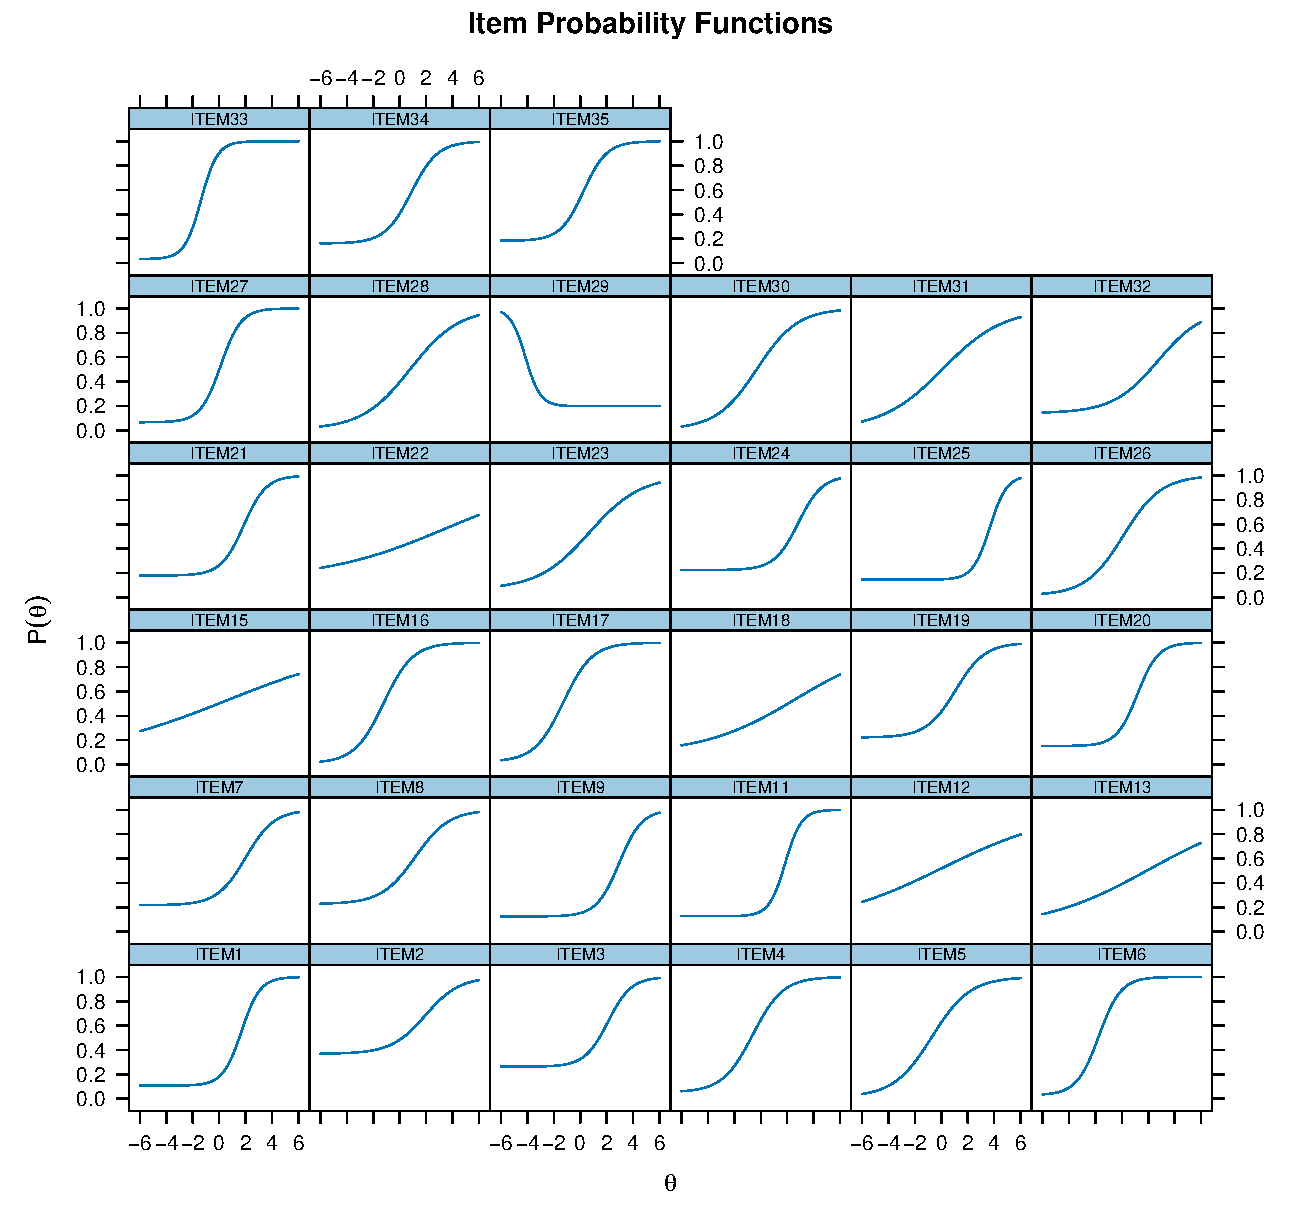
\includegraphics[width=\textwidth,height=0.89\textheight,keepaspectratio]{Curva_Caracteristica1.pdf}
       % \caption{Probabilidade condicional de acerto pelo traço latente. O ponto de inflexão reflete o $b_i$ da dificuldade.}
    \end{figure}
\end{frame}

\begin{frame}{Curvas de Informação dos Itens (CII)}
    \begin{figure}[H]
        \centering
        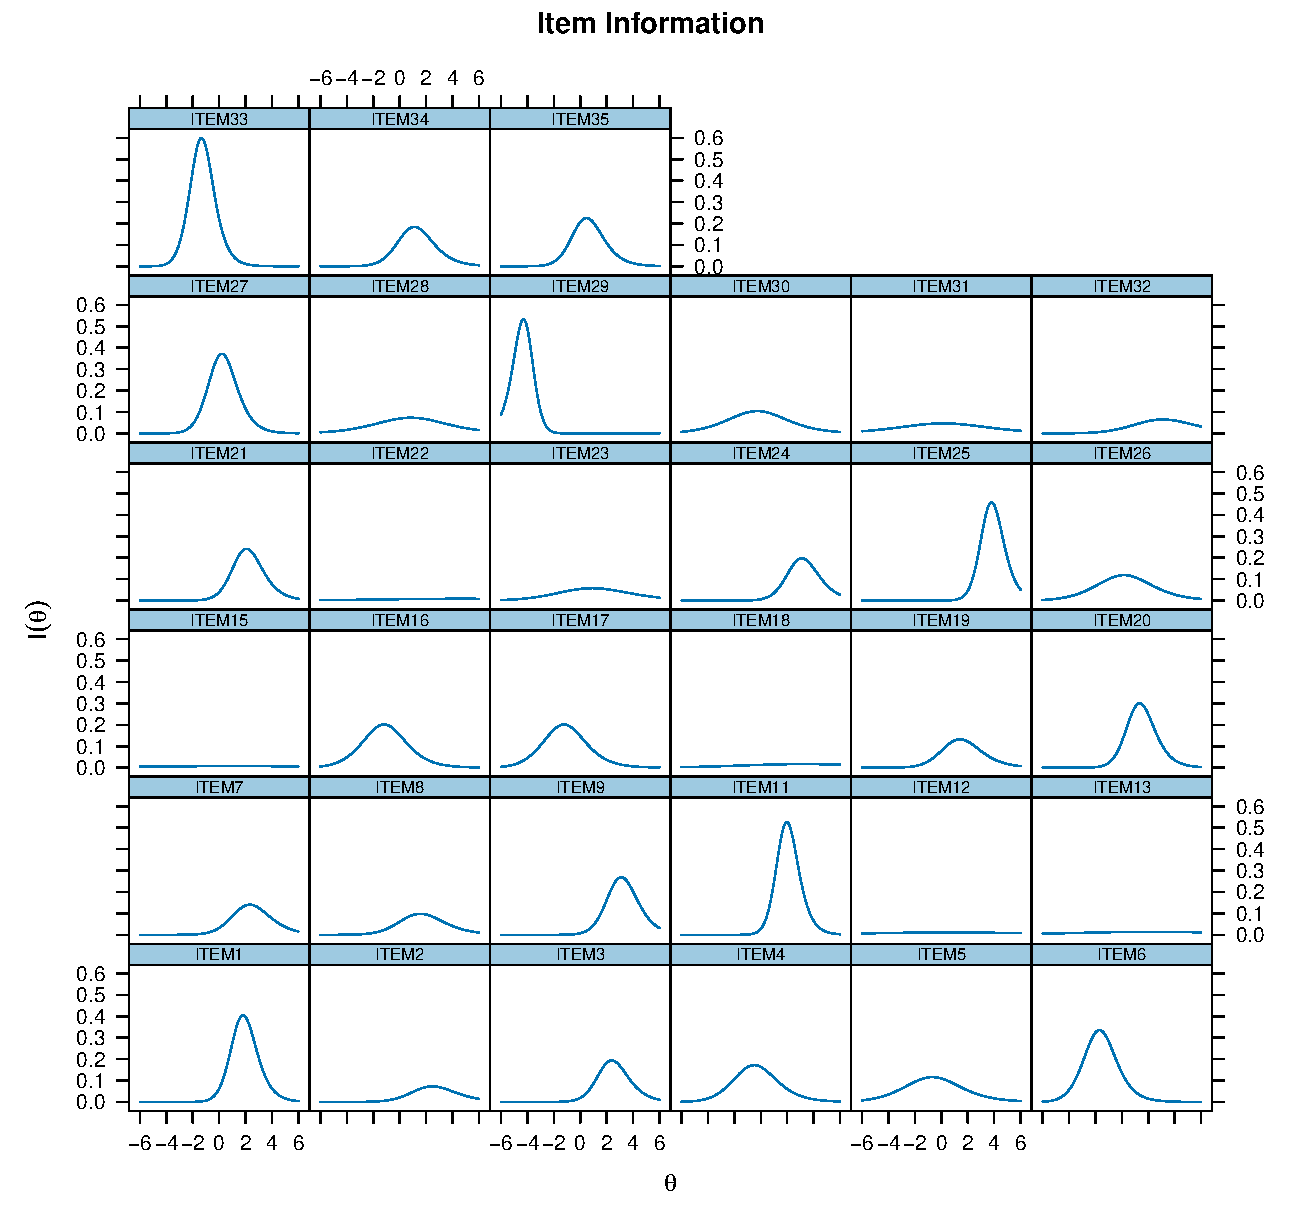
\includegraphics[width=\textwidth,height=0.89\textheight,keepaspectratio]{curva_informacao1.pdf}
       % \caption{Os itens Q33, Q11 e Q01 forneceram o maior montante de informação psicométrica ao modelo.}
    \end{figure}
\end{frame}

\begin{frame}{Curva de Informação Total do Teste (CIT)}
    \begin{figure}[H]
        \centering
        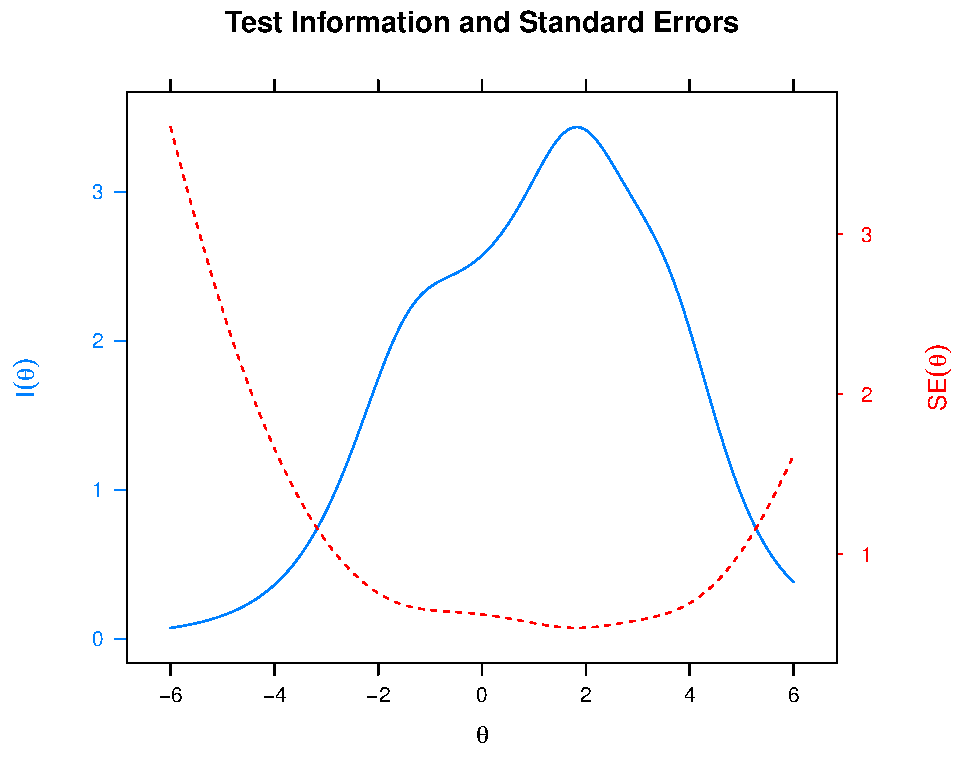
\includegraphics[width=\textwidth,height=0.85\textheight,keepaspectratio]{curva5.pdf}
        %\caption{O teste concentrou sua precisão para alunos de nível Intermediário a Avançado (proficiência de 0 a 4).}
    \end{figure}
\end{frame}

\begin{frame}{Histograma de Proficiência ($\theta$)}
    \begin{figure}[H]
        \centering
        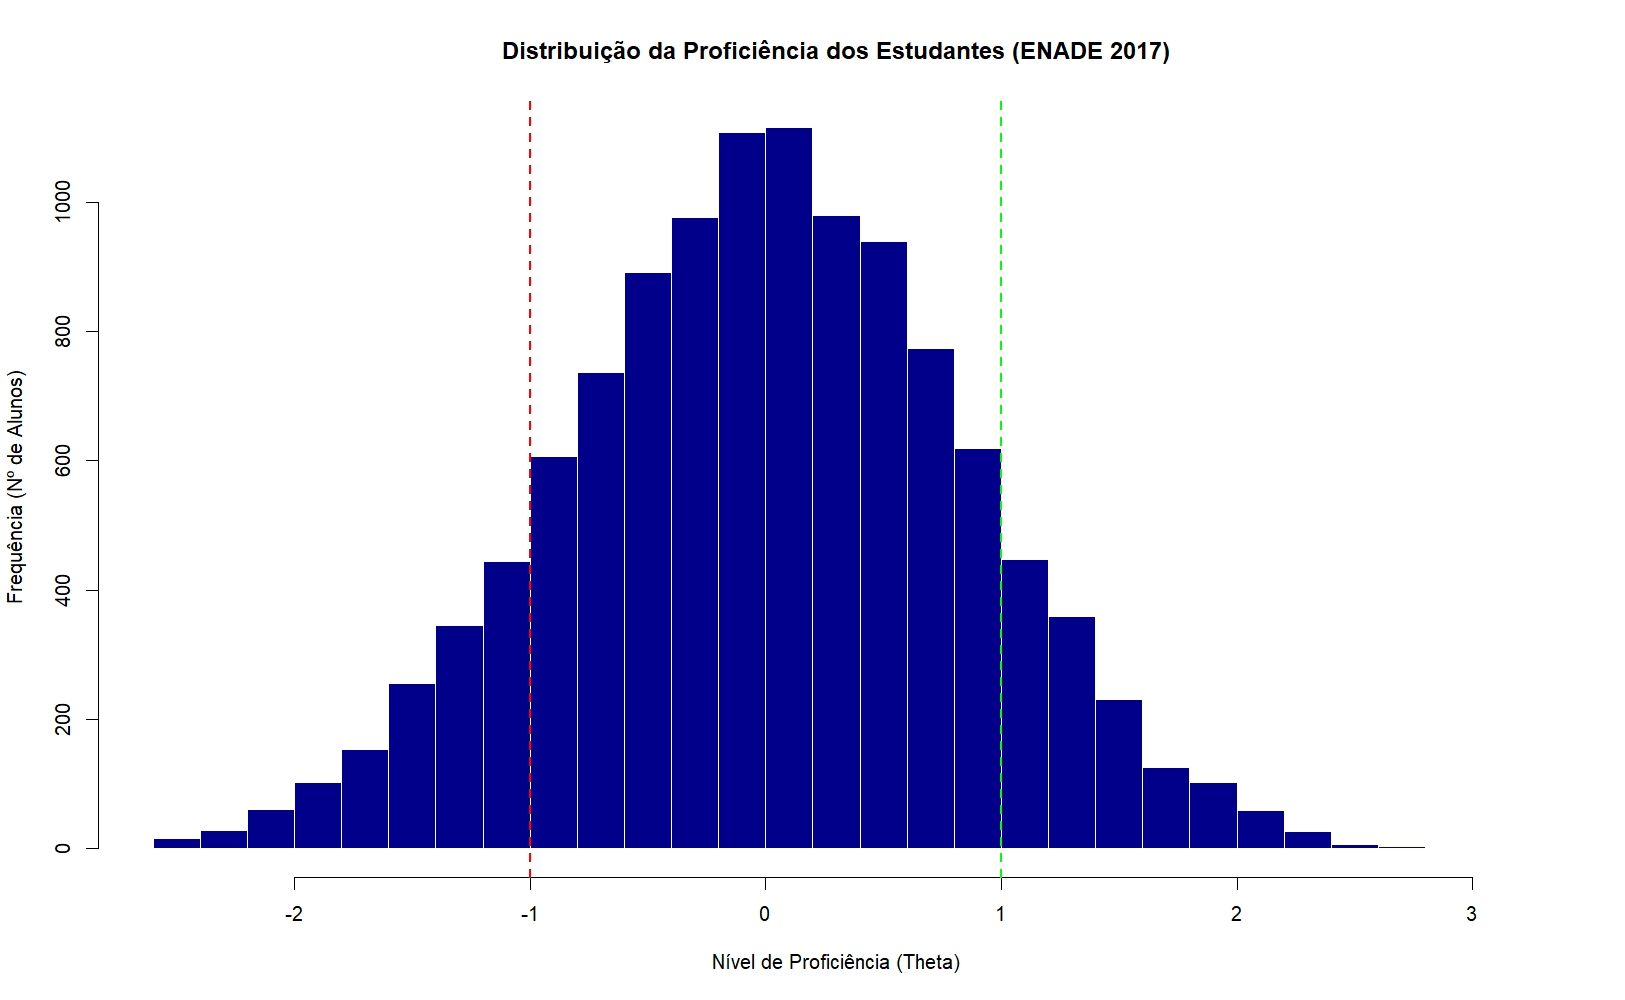
\includegraphics[width=\textwidth,height=0.85\textheight,keepaspectratio]{histograma_proficiencia1.jpeg}
        %\caption{Distribuição dos Estudantes: Básico (12,20\%), Intermediário (75,94\%) e Avançado (11,86\%).}
    \end{figure}
\end{frame}

\begin{frame}{Mapa de Ancoragem de Itens (Mapa de Wright)}
    \begin{figure}[H]
        \centering
        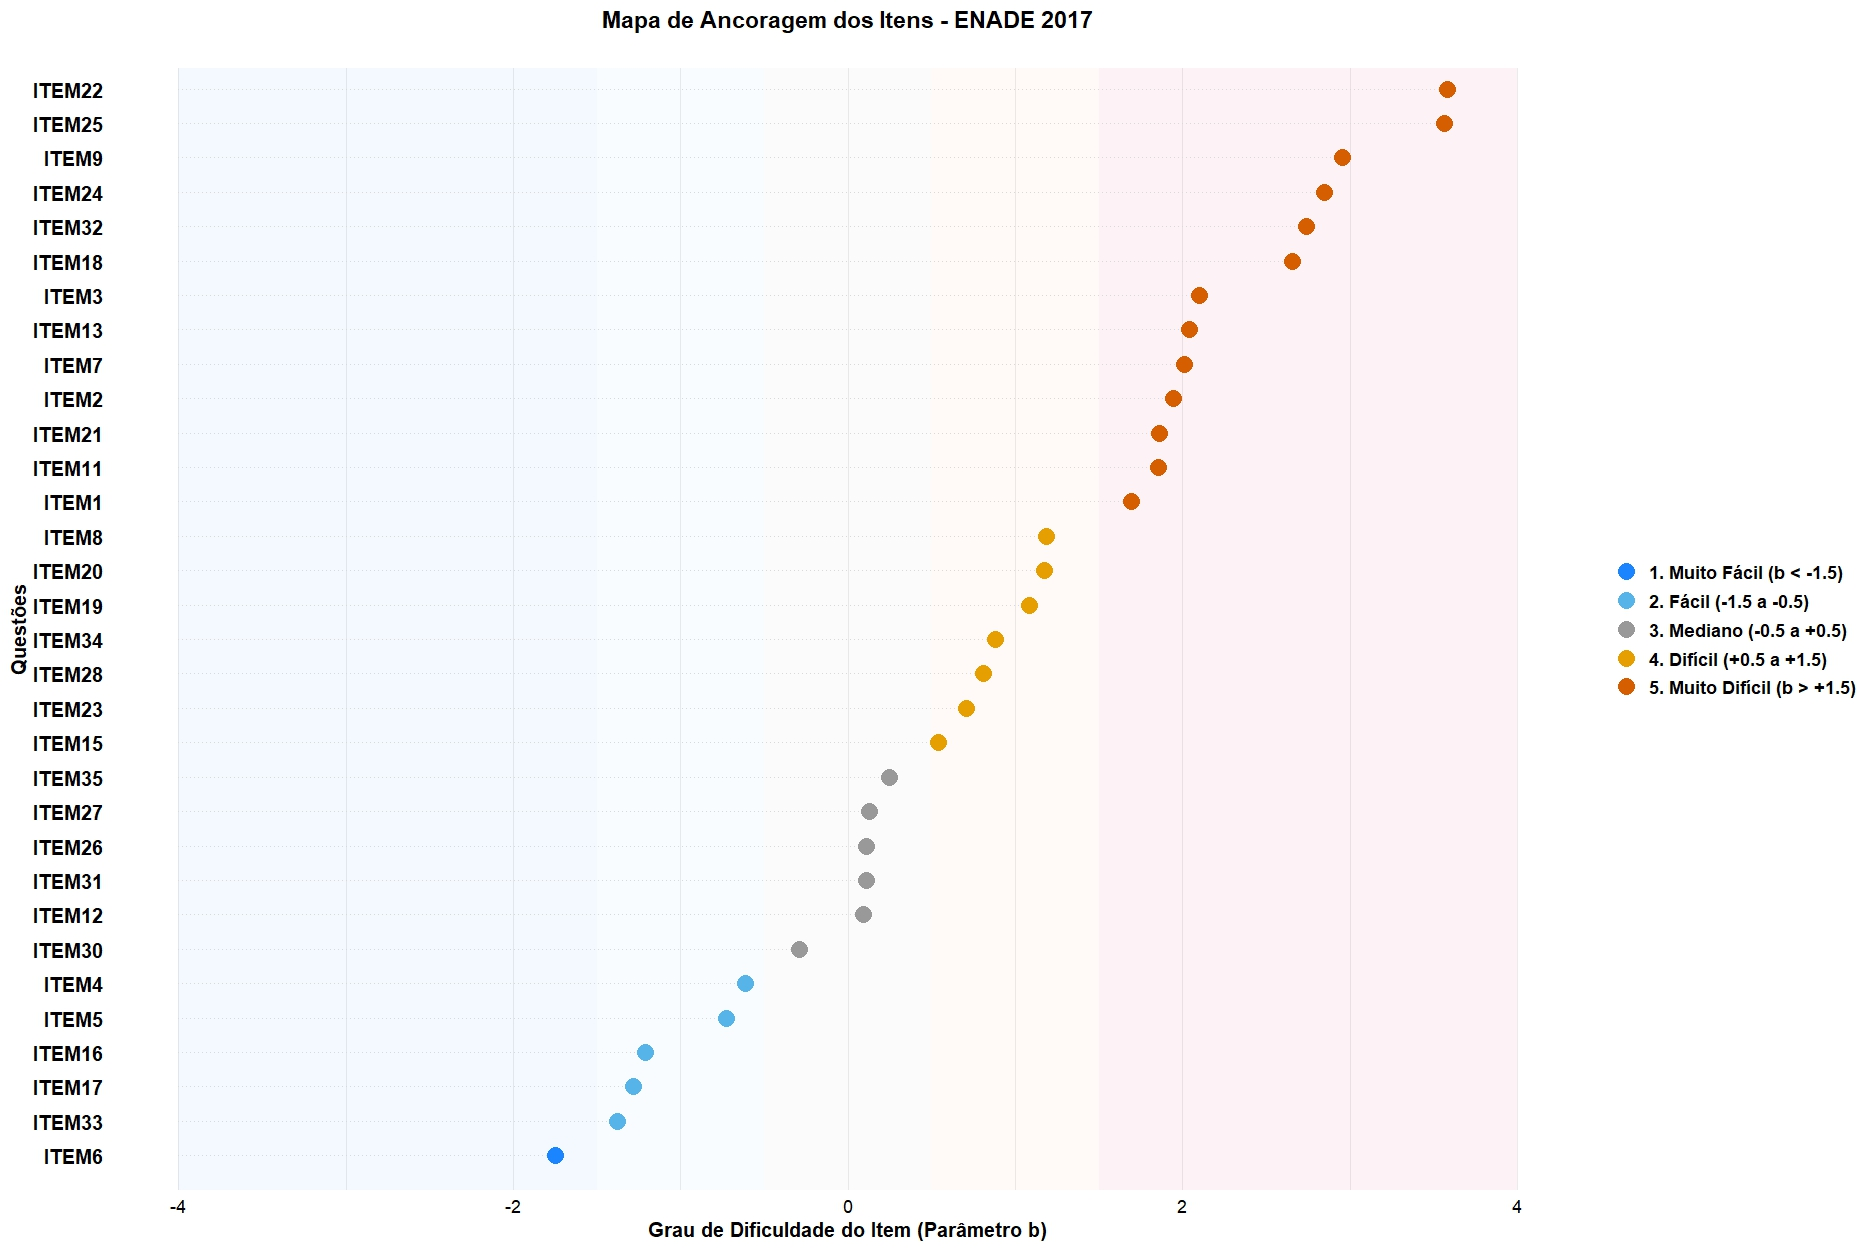
\includegraphics[width=\textwidth,height=0.84\textheight,keepaspectratio]{mapa_aconragem2.jpeg}
       % \caption{A barreira técnica: disciplinas algorítmicas rigorosas separam o aluno mediano do perfil de elite.}
    \end{figure}
\end{frame}

% ==========================================
% SEÇÃO 7: CONCLUSÕES
% ==========================================
\section{Considerações Finais}

\begin{frame}{Considerações Finais}
    \begin{itemize}
        \item \textbf{Eficácia da TRI:} A modelagem capturou perfeitamente os gargalos cognitivos, superando o viés do "acerto casual" que limitava a Teoria Clássica dos Testes.
        \item \textbf{Diagnóstico Curricular:} Disciplinas baseadas no núcleo duro da Computação (Teoria dos Grafos, Algoritmos Avançados, Lógica Discreta) constituem o maior déficit formativo em escala nacional.
        \item \textbf{Ações Institucionais:} As instituições de ensino (IES) devem utilizar essas métricas não apenas para avaliação, mas para \textbf{reestruturação proativa dos PPCs}, fortalecendo a matemática discreta nos semestres iniciais.
    \end{itemize}
\end{frame}

\begin{frame}{Trabalhos Futuros}
    A pesquisa abre caminho para as seguintes expansões analíticas:
    \vspace{0.3cm}
    \begin{enumerate}
        \item \textbf{Modelagem Multidimensional da TRI:} Estimar traços latentes separados para diferentes eixos de formação (ex: eixo algorítmico-matemático \textit{vs.} eixo sociotécnico).
        
        \item \textbf{Aplicação de Machine Learning Supervisionado:} Utilizar a proficiência ($\theta$) extraída neste trabalho de forma não-supervisionada como variável alvo (\textit{target}). Assim, pode-se treinar algoritmos (ex: Random Forest, \textbf{XGBoost}) usando os dados socioeconômicos do ENADE (renda, cota, etc.) como \textit{features} para prever o desempenho do aluno.
        
        \item \textbf{Análise Longitudinal Pós-DCNs:} Comparar este \textit{baseline} de 2017 com os ciclos do ENADE de 2021, 2024 e 2026 para auditar se a implantação de novas Diretrizes Curriculares gerou impactos concretos na proficiência.
    \end{enumerate}
\end{frame}

% --- SLIDE FINAL ---
\begin{frame}
    \centering
    \Huge \textbf{Muito Obrigado!}
    
    \vspace{1cm}
    \large \textbf{Mário Diego Rocha Valente} \\
     \large \textbf{Dionne Cavalcante Monteiro} \\
    \large \textbf{Heliton Ribeiro Tavares}
\end{frame}

\end{document}